\documentclass[12pt,oneside,a4paper]{article}
\usepackage[utf8x]{inputenc}
\usepackage[T1]{fontenc}
\usepackage[english,polish]{babel}
\usepackage{polski}
\usepackage{listings}
\usepackage{amstext}
\usepackage{float}
\usepackage{longtable}
\restylefloat{table}
\usepackage[top=2.5cm,bottom=2.5cm,left=3.5cm,right=2.5cm]{geometry}
\usepackage{indentfirst}
\usepackage{graphicx}
\usepackage{enumitem}
\usepackage{tabularx}
\usepackage{hyperref} %spis treści niech będzie łączami
\hypersetup{
	plainpages=false,
    colorlinks,
    citecolor=black,
    filecolor=black,
    linkcolor=black,
    urlcolor=black
}
\linespread{1.3}
\setlength{\parindent}{4ex}
\begin{document}
\author{Marcin Kubik}
\author{Jacek Sosnowski}
\author{Jacek Witkowski}
\author{Piotr Zapaśnik}
\title{APSI - sklep rowerowy}
\pagenumbering{alph}
\begin{titlepage}
    \vbox to\textheight{\hyphenpenalty=10000
    \begin{center}
	\begin{tabular}{p{107mm} p{9cm}}
	    \begin{minipage}{9cm}
	      \begin{center}
	      Politechnika Warszawska \\
	      Wydział Elektroniki i~Technik Informacyjnych \\
	      Instytut Informatyki
	      \end{center}
	    \end{minipage}
	    &
	    \begin{minipage}{8cm}
	    \begin{flushleft}
	     \footnotesize
	      Rok akademicki 2013/2014
	    \vspace*{2.75\baselineskip}
	    \end{flushleft}
	    \end{minipage} \\
	\end{tabular}
	\vspace*{0.75\baselineskip}
	\par\vspace{\smallskipamount}
	{\strut Marcin Kubik\par}
	{\strut Jacek Sosnowski\par}
	{\strut Jacek Witkowski\par}
	{\strut Piotr Zapaśnik\par}
	\vspace*{1\baselineskip}{\LARGE ANALIZA I PROJEKTOWANIE SYSTEMÓW
	INFORMACYJNYCH\par}

	\vspace*{2\baselineskip}{\huge\bfseries Internetowy sklep rowerowy\par}

	\vspace*{2\baselineskip}
	\hfill\mbox{}\par\vspace*{\baselineskip}\noindent
	\begin{tabular}[b]{@{}p{3cm}@{\ }l@{}}
	    {\large\hfill } & {\large }
	\end{tabular}
	\hfill
	\begin{tabular}[b]{@{}l@{}}
	Prowadzący: \\[\smallskipamount]
	{\large mgr inż. Piotr Salata}
	\end{tabular}\par
	\vspace*{2\baselineskip}
    \begin{tabular}{p{\textwidth}}
    \end{tabular}
    \end{center}} 

\end{titlepage}
\clearpage
\tableofcontents
\pagenumbering{arabic}
\clearpage
\section{Wstęp}

Tutaj będzie wstęp\ldots
\section{Zakres realizacji}

Niniejszy rozdział prezentuje specyfikację wymagań odnośnie sposobu realizacji
projektu. Nakreślając role poszczególnych zespołów oraz główne zadania jakie
mają realizować w ramach swoich prac.

\subsection{Realizacja projektu}

Projekt jest realizowany w siedzibie firmy Bike Shop sp. z.o.o.
Umożliwi to szybkie podejmowanie decyzji w przypadku powstawania
ewentualnych niejasności a także łatwiejsze reagowanie na przeszkody,
jakie pojawiają się w czasie procesu projektowania. 
Zleceniodawca zobowiązał się do delegacji doświadczonego pracownika, który zna
specyfikę działania firmy oraz jej cele biznesowe. Ta osoba będzie uczestniczyć
w projekcie bezpośrednio na etapie analizy.

Zgodnie z dokumentem załączonym do umowy Zleceniodawca zobowiązał się do
udostępnienia firmie implementującej system pomieszczenia, w których
możliwa będzie praca zespołu projektowego. Pomieszczenia takie
powinny charakteryzować się dostępem do szybkiego łącza
internetowego. 

\subsection{Wstępny zarys technologiczny}
Tworzony przez zleceniobiorcę system zostanie stworzony w logice
trójwarstwowej umożliwiającej łatwe i wydajne zarządzanie całością
przedsięwzięcia oraz umożliwiającej dalszą modyfikację i rozbudowę.
Podział na warstwy jest następujący:

\begin{itemize}
  \item Warstwa prezentacji odpowiada za część graficzną, reprezentację danych
  przechowywanych w systemie oraz za umożliwienie użytkownikowi przeglądania
  dostępnych produktów, a także złożenie zamówienia. Osobny moduł odpowiedzialny
  jest za dostęp do administracyjnych części systemu, dostępny wyłącznie dla
  pracowników firmy Bike Shop z.o.o.
  \item Serwer aplikacji zawierający logikę tworzonego systemu, odpowiedzialny
  za zarządzanie zamówieniami, komunikację pomiędzy bazą danych oraz interfejsem
  klienckim a także wykorzystanie infrastuktury internetowej w celu zwiększenia
  wydajności
  \item Baza danych przechowująca informacje na temat wszystkich produktów
  dostępnych w sklepie, klientów posiadających swoje konta oraz składanych przez
  nich zamówieniach.
\end{itemize}

Proces projektowy systemu zostanie oparty o dwa niezależne zespoły (analityczne
i projektowe)

\subsection{Analitycy - wymagania}
Zespół ten w ramach projektu zajmuje się prowadzeniem analizy biznesowej,
badaniem potrzeb klientów, projektuje rozwiązania dla systemu. Jest
odpowiedzialny za określanie wymagań (zarówno funkcjonalnych jak i
niefunkcjonalnych). Jego zadaniem jest też dbałość o ich prawidłową realizację.

Główne zadania:

\begin{itemize}
  \item Określenie wymagań stawianych przed systemem
  \item Tworzenie specyfikacji wymagań
  \item Tworzenie planu testów
  \item Analiza środowiska systemowego
  \item Tworzenie dokumentów projektowych
  \item Odpowiedzi na wątpliwości powstałe na etapie projektowania, czy
  implementacji
\end{itemize}

\subsection{Projektanci - wymagania}
Zespół jest odpowiedzialny za stworzenie architektury nowopowstającego
systemu oraz zapisanie jej w postaci dokumentacji technicznej. Wyniki prac tego
zespołu są niezbędne dla późniejszych etapów. W czasie implementacji służą jako
wsparcie dla programistów tworzących system.

Główne zadania:

\begin{itemize}
  \item Tworzenie projektu systemu informatycznego (oddzielnie projekt
  architektury i bazy danych)
  \item Wybór technologii i metod realizacji systemu
  \item Tworzenie dokumentacji technicznej wykorzystywanej podczas implementacji
  \item Bieżące dostosowywanie wymagań do postępów prac
\end{itemize}
\newpage
\section{Wymagania}

W tej sekcji znajduje się lista wymagań jakie spełniać powinien budowany system.
Podane są one z podziałem na dwie kategorie. Pierwsza to wymagania funkcjonalne
określające funkcjonalności systemu oraz sposoby ich użycia. Druga natomist to
wymagania niefunkcjonalne, które opisują ilościowe i jakościowe warunki
działania systemu.

\subsection{Wymagania funkcjonalne}
\subsubsection{Zamówienia}

Wymagania funkcjonalne dotyczące zamówień realizowanych przez sklep:

\begin{enumerate}
  \item Prezentacja zamówień
  \item Edycja, modyfikacja
  \begin{enumerate}
    \item Dodanie lub usunięcie produktu z zamówienia
    \item Zmiana ilości produktu
  \end{enumerate}
  \item Zmiana danych zamawiającego
  \item Usunięcie zamówienia w całości
  \item Edycja formy płatności
  \begin{enumerate}
    \item Płatność gotówką
    \begin{enumerate}
      \item Koszt w złotówkach
      \item Koszt w euro
      \item Koszt w wirtualnej walucie
    \end{enumerate}
    \item Płatność przelewem
    \item Płatność ratalna oparta o system szybkich pożyczek SuperBank
    \item Możliwość wpłaty zaliczki przed wysyłką
    \item Obniżenie kosztu o naliczone rabaty i zniżki
  \end{enumerate}
  \item Wybór sposobu potwierdzenia zamówienia (faktura, paragon)
  \item Generowanie faktury pro-forma dla danego zmówienia
  \item Zarządzanie terminem dostawy
  \item Ustawianie aktualnego stanu zamówienia.
\end{enumerate}
\subsubsection{Klient}

Wymagania funkcjonalne dotyczące klientów zamawiających części w sklepie

\begin{enumerate}
  \item Dodanie nowego klienta
  \item Edycja danych klienta
  \begin{enumerate}
    \item Edycja adresu klienta
    \item Edycja adresu e-mail
  \end{enumerate}
  \item Edycja czułych danych klienta
  \begin{enumerate}
    \item Edycja hasła
    \item Edycja statusu (stały klient, nowy klient)
  \end{enumerate}
  \item Wyrejestrowanie się klienta
  \item Usunięcie klienta
\end{enumerate}

 
\subsubsection{Opis przypadków użycia - klient}

Opis przypadków użycia wyjaśniające funkcjonalności związane z zarządzaniem
klientami:

\begin{enumerate}
  \item Rejestracja klienta \\
  \begin{tabularx}{\linewidth}{ c X }
  Aktor: & Klient \\
  Opis: & Możliwość rejestracji nowego klienta.\\
  \end{tabularx}
   \begin{enumerate}
    \item Klient uruchamia stronę internetową sklepu i wybiera opcję rejestracji
    \item Klient wstawia swoje dane osobowe i wybiera domyślny model płatności
    (kartą, za pobraniem itp.)
    \item System sprawdza wstawione dane (takie same hasła, czy istnieje już
    zarejestrowany w systemie użytkownik, czy istnieje podany adres e-mail itp.)
    \item System wysyła e-mail powitalny na adres podany przez klienta
    \item W ciągu określonego, zdefiniowanego czasu klient wybiera przesłany w
    e-mailu link, stając się pełnoprawnym użytkownikiem sklepu
  \end{enumerate}
  \item Złożenie zamówienia \\
  \begin{tabularx}{\linewidth}{ c X }
  Aktor: & Klient \\
  Opis: & Przedstawienie sposobu złożenia zamówienia.\\
  \end{tabularx}
  \begin{enumerate}
    \item Klient uruchamia stronę internetową sklepu i wyszukuje interesujące go
    produkty
    \item W momencie znalezienia pasującego produktu użytkownik wybiera opcję
    dodania do koszyka
    \item Po zakończeniu wyszukiwania użytkownik wybiera opcję przejścia do kasy
    \item System sprawdza, czy użytkownik jest zalogowany. Jeśli nie, procesuje
    przypadek użycia Logowanie do Systemu
    \item System sprawdza, czy użytkownik jest stałym klientem. Jeśli tak,
    dolicza rabat do ustalonej ceny (do sumy cen poszczególnych produktów)
    \item Użytkownik wybiera sposób płatności
    \item System dodaje do wcześniej ustalonej ceny koszty wynikające ze sposobu
    płatności
    \item Użytkownik wybiera sposób dostawy (poczta, kurier, odbiór osobisty
    itp.)
    \item System dodaje do ceny koszty wynikające ze sposobu dostawy
    \item Użytkownik, po sprawdzeniu wszystkich danych, decyduje się na złożenie
    zamówienia - po tym momencie nie może już ono być cofnięte
    \item System wysyła do użytkownika e-mail potwierdzający wraz z przewidywaną
    datą realizacji zamówienia
  \end{enumerate} 
  \item Edycja danych klienta \\
  \begin{tabularx}{\linewidth}{ c X }
  Aktor: & Klient \\
  Opis: & Możliwość zmiany, uzupełnienia danych osobowych klienta.\\
  \end{tabularx}
  \begin{enumerate}
    \item Klient uruchamia witrynę internetową sklepu
    \item Klient loguje się do systemu (tylko osoba zalogowana może zmieniać
    swoje dane)
    \item Klient edytuje wybrane pozycje ze swojego opisu (adres, numer
    telefonu itp.)
    \item W przypadku zmiany hasła klient proszony jest o podanie starego jak i
    nowego (dwukrotnie) hasła
    \item Klient zatwierdza wprowadzone zmiany
    \item System wysyła na podany przez użytkownika adres e-mail (nowy, jeśli
    to adres e-mail był jedną ze zmienianych wartości) informację o zmianie.
  \end{enumerate}
  \item Wyrejestrowanie się klienta \\
  \begin{tabularx}{\linewidth}{ c X }
  Aktor: & Klient \\
  Opis: & Klient ma możliwość w każdym momencie usunąć swoje konto z systemu.\\
  \end{tabularx}
  \begin{enumerate}
    \item Klient uruchamia witrynę internetową i loguje się na swoje konto
    (przypadek użycia Logowanie Do Systemu)
    \item Klient wybiera opcję usunięcia danych
    \item System sprawdza, czy istnieją niezrealizowane (oczekujące) zamówienia.
    Jeśli tak, wyświetla się alert z informacją, czy dane zamówienie zostało już
    wcześniej opłacone
    \item Jeśli istniały już zamówienia, które zostały opłacone a nie zostały
    jeszcze zrealizowane, system zleca odesłanie określonej kwoty pieniężnej z
    powrotem na konto użytkownika (z pominięciem kosztów obsługi)
    \item Klient zostaje poproszony o podanie przyczyn swojej decyzji -
    wypełnianie jest nieobowiązkowe
    \item Dane przechowywane są przez Okres Przechowywania Danych (wymaganie
    prawne - patrz Wymagania niefunkcjonalne punkt \ref{itm:OPD}). W tym
    czasie klient może ponownie zarejestrować się w systemie bez utraty poprzednich danych
    \item W przypadku braku ponownej rejestracji dane zostają na stałe usunięte
    z firmowej bazy danych
  \end{enumerate}
  \item Usunięcie klienta \\
  \begin{tabularx}{\linewidth}{ c X }
  Aktor: & Pracownik \\
  Opis: & Klienta można usunąć administracyjnie na przykład z powodów
  naruszenia regulaminu.\\
  \end{tabularx}
  \begin{enumerate}
    \item Pracownik sklepu wyszukuje klienta o konkretnym imieniu i nazwisku
    (lub według innych kryteriów)
    \item Pracownik wybiera opcję usunięcia klienta. 
    \item Pracownik wpisuje powód, dla którego usuwa użytkownika (informacja ta
    będzie przesłana do klienta w wiadomości e-mail)
    \item Pracownik wypełnia dane dotyczące kwestii niezrealizowanych zamówień i
    nieotrzymanych płatności
    \item Obie informacji (z poprzednich 2 kroków) są przekazywane na podany
    przez użytkownika adres e-mail
    \item Dane są przechowywane przez Okres Magazynowania Danych (patrz
    Wymagania Niefunkcjonalne punkt \ref{itm:OMD}) - w tym czasie użytkownik
    może złożyć reklamację i ewentualnie odzyskać dostęp do konta
    \item Po tym czasie, jeśli prośba o przywrócenie konta nie zostanie
    pozytywnie rozpatrzona, dane są na stałe usuwane z systemu
  \end{enumerate}
\end{enumerate}
\newpage
\subsection{Wymagania niefunkcjonalne}

\begin{enumerate}
  \item Pojemność: \\ 
  System powinien mieć możliwość przechowywania danych o 100 tys.
  użytkowników 
  \item Wydajność: \\ 
  System powinien obsługiwać bez znaczącego spadku wydajności 400
  użytkowników ``jednocześnie''. Zakładając, że użytkownik będzie wymagał
  maksymalnie 20 odświeżeń widoku systemu na minutę (jedna podstrona na 3
  sekundy). System powinien działać z wydajnością 8000 odświeżeń/minutę. 
  \item System powinien być dostępny dla klientów 24 godziny na dobę 7 dni w
  tygodniu (możliwe są przerwy konserwacyjne, jednak nie dłuższe niż 4 godziny na miesiąc pracy) 
  \item Średni czas naprawy (MTTR - ang. Mean Time to Recover) na poziomie
  1~godziny
  \item System powinien umożliwiać klientom dostęp z dowolnego miejsca na
  świecie za pomocą sieci Internet oraz jego działanie powinno być niezależne od
  używanej platformy systemowo-sprzętowej użytkownika.
  \item Dane osobowe muszą być przetwarzane zgodnie z ustawą o ochronie danych
  osobowych z dnia 29 sierpnia 1997 r. 
  \item Klient powinien mieć dostęp do wszystkich swoich danych (łącznie z
  możliwością ich aktualizacji i usunięcia) zgodnie z polskim prawem
  \item Dane te powinny być chronione w zależności od ich poziomu poufności
  (dane do autoryzacji powinny być zabezpieczone przed możliwością odczytu nawet
  przez administratora) 
  \item Komunikacja pomiędzy klientem (przeglądarką internetową, aplikacją
  mobilną itp.) powinna być szyfrowana w sposób uniemożliwiający odczytanie czułych informacji
  \item System powinien mieć wbudowane procedury przeciwdziałania sytuacjom
  awaryjnym - procedury uruchamiane przez administratora
  \begin{enumerate}
    \item Procedury sprawdzenia spójności danych - po odzyskaniu sprawności, np.
    po awarii sprzętu
    \item Procedury uruchamiane w przypadku wykrycia włamania (między innymi,
    odłączenie systemu od sieci Internet, zablokowanie modyfikacji elementów
    systemu itp.)
  \end{enumerate} 
  \item System posiadać będzie hierarchię uprawnień (ról) dla użytkowników,
  przydzielanych im w celu umożliwienia korzystania z dodatkowych
  funkcjonalności
  \item System domyślnie powinien nadawać użytkownikowi uprawnienia nie większe
  niż niezbędne mu do poprawnego zamawiania produktów i zarządzania swoim
  kontem
  \item System powinien umożliwiać automatyczne wysyłanie klientowi wiadomości
  e-mail (z prośbą o potwierdzenie zmiany hasła czy akceptacji warunków rejestracji)
  \item System powinien umożliwiać użytkownikowi zmianę (w ograniczonym stopniu)
  już złożonego zamówienia (zmiana adresu przed wysyłką itp.) bez konieczności
  ingerencji pracownika sklepu
  \item System powinien być zdolny do wyświetlania informacji w wielu językach.
  Początkowo będzie to język polski i angielski. Istnieje jednak możliwość
  rozszerzenia o kolejne.
  \item \label{itm:OPD} Okres Przechowywania Danych - to czas przez który będą
  przechowywane dane użytkownika sprzed ich zmiany lub wyrejestrowania - system zapewnia
  magazynowanie tych danych co najmniej przez 7 dni.
  \item \label{itm:OMD} Okres Magazynowania Danych to czas 30 dni przez które
  system powinien przechowywać dane o klientach po usunięciu konta klienta (czas ten może się
  zmienić z powodów prawnych)
  \item \label{itm:Platnosci} System wspiera następujące formy płatności:
  \begin{enumerate}
    \item Płatność gotówką
    \item Przelew bankowy
    \item Płatność ratalna w oparciu o zewnętrzną usługę bankową
  \end{enumerate}
  Waluty: polski złoty, euro, bitcoin
  \item \label{itm:PotwierdzenieTransakcji} Forma potwierdzenia transakcji:
  faktura albo paragon
  \\
  System powinien umożliwiać generowanie tych dokumentów oraz ich wydruk.
  
\end{enumerate}

\newpage
\section{Model analityczny}

Celem stworzonego w niniejszym rozdziale modelu analitycznego jest
zdefiniowanie, jak wyglądać będzie architektura tworzonego systemu, jakie
problemy mogą być związane z poszczególnymi elementami całości i jakie kroki
można przedsięwziąć w celu zapobieżenia najczęściej występującym i najbardziej
prawdopodobnym zagrożeniom. Aby to osiągnąć, zaprezentowano różnego rodzaju
diagramy UML, które służą jako wizualna reprezentacja architektury systemu i
pozwalają na łatwiejszą analizę stanu projektu.


Przedstawiony na poniższym obrazku diagram klas reprezentuje wszystkie
wykorzystywane przez Zleceniodawcę elementy składające się na cały system.
Diagram ten ma znaczenie przede wszystkim dla deweloperów i osób zajmujących się
wytwarzaniem oprogramowania, tym niemniej powinien zostać zatwierdzony przed
przedstawicieli Zleceniodawcy - diagram klas jest bowiem punktem łączącym z
jednej strony wyobrażenie klienta o podziale funkcjonalności a z drugiej decyzje
projektowe podjęte przez zespół zajmujący się implementacją.

Diagram klas powinien obrazować zależności (agregacje, kompozycje, relację
dziedziczenia) pomiędzy poszczególnymi klasami na tyle szczegółowo, by osoby 
nieposiadające wykształcenia informatycznego i nieznające metod programowania
obiektowego mogłby zrozumieć zasadę podziału bez szczegółowych wyjaśnień. Z
tego też powodu na poniższym rysunku skoncentrowano się na powiązaniach pomiędzy
poszczególnymi klasami a nie na nazywaniu i przedstawianiu atrybutów i metod
poszczególnych klas. Nie stanowią one żadnej wartości z punktu widzenia
Zleceniodawcy a mogą stanowić ograniczenie i usztywnienie schematu dla
deweloperów, którzy lepiej znają metody dostarczania funkcjonalności i będą
mogli lepiej modyfikować schemat w zależności od potrzeb, nie naruszając
jednocześnie warunków umowy. Wszystkie atrybuty czy operacje ważne z punktu
widzenia Zleceniodawcy, które mogą mieć wpływ na ocenę projektu zostały
umieszczone na diagramie.

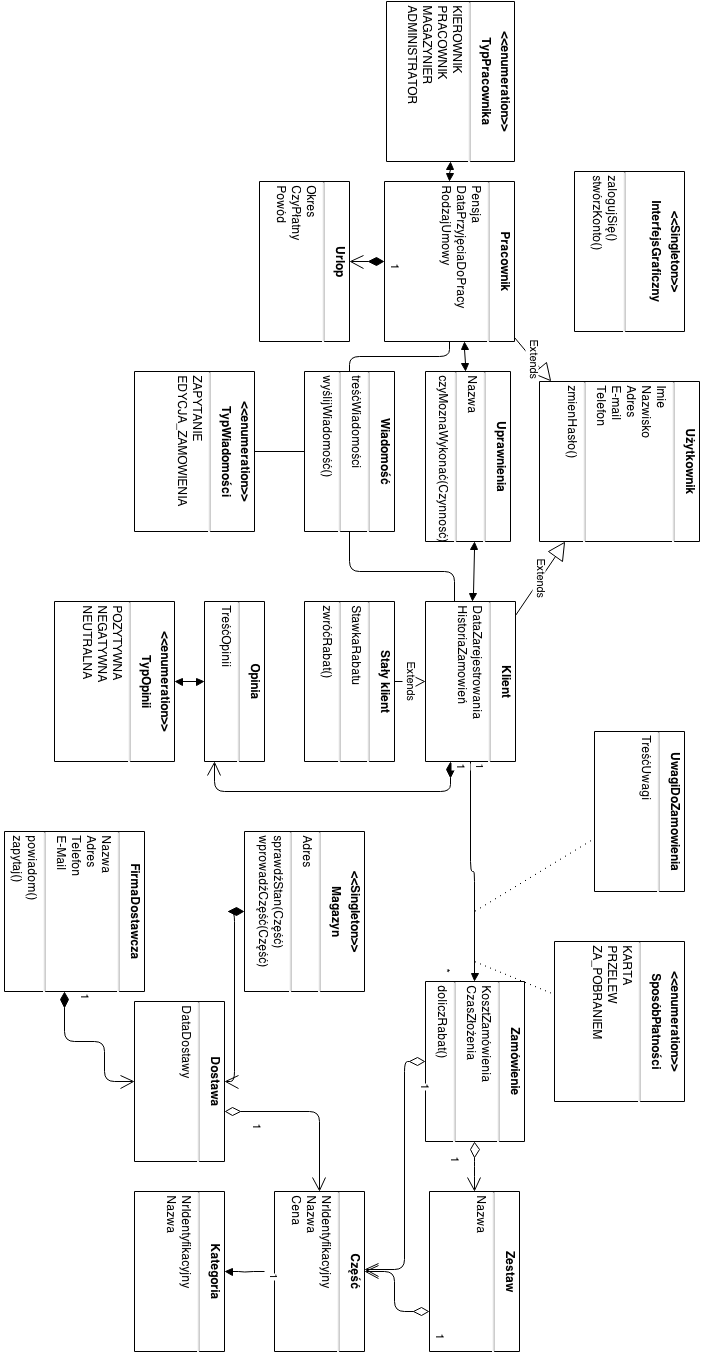
\includegraphics[width=\textwidth,
height=0.8\textheight]{graphics/ClassDiagram.png}


\newpage
Opis klas na przedstawionym diagramie:

\begin{description}
	\item[Użytkownik] \hfill \\
		Klasa abstrakcyjna, będąca bazową dla klas Klient i Pracownik, przechowuje
		informacje dotyczące danej osoby - imię, nazwisko, adres e-mail itp.
	\item[Pracownik] \hfill \\
	 	Osoba z obsługi sklepu, odpowiedzialna za realizację i zarządzanie
	 	zamówieniami
	\item[Stały klient] \hfill \\
		Osoba charakteryzująca się dużą liczbą zamówień bądź długim czasem obecności
		na stronie (czas liczony od czasu rejestracji)
	\item[Klient] \hfill \\
		Osoba składająca zamówienia w sklepie, edytująca swoje zamówienia i opłacająca
		je
	\item[Typ pracownika] \hfill \\
		Enumeracja, będąca oznaczeniem rodzaju pracownika (Szeregowy Pracownik,
		Kierownik itp.)
	\item[Urlop] \hfill \\
		Obsługa urlopów dla pracowników pod kątem czasu ich trwania, momentu ich
		rozpoczęcia (i zakończenia) itp.
	\item[Uprawnienia] \hfill \\
		Obsługa uprawnień zarówno dla pracowników jak i klientów. Pozwala na
		ustalanie, kto ma jakie uprawnienia do edycji i podglądu danych
	\item[Wiadomość] \hfill \\
		Treści przesyłane pomiędzy pracownikami i klientami, służące do przekazywania
		informacji na temat zamówień
	\item[Typ wiadomości] \hfill \\
		Enumeracja, jaki rodzaj wiadomości jest przekazywany (Zapytanie, Edycja
		Zamówienia itp.)
	\item[Opinia] \hfill \\
		Tekst na temat zamówienia, ocena poprawności i jakości realizacji zamówienia
	\item[Typ opinii] \hfill \\
		Enumeracja, jaka opinia została wydana (Pozytywna, Negatywna, Neutralna)
	\item[Zamówienie] \hfill \\
		Informacje na temat złożonego przez klienta Zamówienia
	\item[Uwagi do zamówienia] \hfill \\
		Wszelkiego rodzaju informacje, jakie klient chce zawrzeć w momencie złożenia
		zamówienia - na przykład zaznaczanie wysyłki jako prezent, ustalenie, przed
		jakim terminem zamówienie nie powinno być wysłane, czy możliwy jest odbiór
		osobisty itp.
	\item[Sposób płatności] \hfill \\
		Informacja, jak użytkownik chce zapłacić za złożone zamówienie - inaczej
		wygląda procesowanie zapłaty kartą (wysłanie następuje dopiero po wpłynięciu
		pieniędzy, opłata za pobraniem jest uiszczana dopiero po wysłaniu)
	\item[Część] \hfill \\
		Pojedyncza część rowerowa wraz z informacjami na jej temat - rozmiar, nazwa,
		cena itp.
	\item[Zestaw] \hfill \\
		Złożenie kilku części w jeden, funkcjonalnie sprawny rower. Przechowuje
		informację o tym, jakie części są wymagane, ile ma ich być (rama - 1, pedały
		-2, przerzutki - nieokreślone)
	\item[Kategoria] \hfill \\
		Informacja, do jakiej kategorii zaliczana jest dana część. Jest to pomocne do
		układania zestawów i sprawdzania ich poprawności
	\item[Dostawa] \hfill \\
		Informacje na temat jednej dostawy, jakie części i w jakiej ilości zostały
		dostarczone i kiedy
	\item[Firma dostawcza] \hfill \\
		Informacje na temat firmy, która dostarcza części - dane kontaktowe, adres
		oraz jakie części są w stanie dostarczyć
	\item[Magazyn] \hfill \\
		Klasa pozwalająca na zarządzanie częściami przechowywanymi w magazynie,
		sprawdzanie ich dostępności oraz aktualizacja stanu
	\item[Interfejs graficzny] \hfill \\
		Klasa będąca ``wejściem'' do diagramu klas, odpowiedzialna za podstawową,
		wstępną integrację z użytkownikiem
\end{description}
\newpage
\section{Rozwiązania projektowe}

Niniejszy projekt tworzony jest dla klienta zewnętrznego, firmy zajmującej się
dystrybucją i sprzedażą rowerów. Stawiane przed deweloperami wymagania są zatem
podobne do tych, jakie są udziałem większości zespołów zajmujących się
implementacją rozwiązań internetowych. Celem projektu jest stworzenie
internetowego sklepu, który umożliwiałby zarówno kupowanie (zamawianie)
produktów związanych z szeroko pojętą branżą rowerową jak i śledzenie statusu
takich zamówień, zarządzanie nimi oraz ich ewentualne usuwanie. System powinien
także współpracować z pracownikami firmy Bike Shop sp. z.o.o. w zakresie obsługi
nowych dostaw, wprowadzania i zdobywania informacji o zamówieniach oraz kontaktów z
klientami. Działanie systemu można zatem podzielić na dwie główne kategorie:

\begin{description}
	\item[Moduł dla klientów] \hfill \\
	Składanie zamówień, edycja wprowadzonych danych na temat klientów, wydawanie
	opinii na temat sklepu, składanie zapytań
	\item[Moduł dla pracowników]
	Wprowadzanie danych o częściach rowerowych, odpowiadanie na zapytania klientów,
	informowanie o statusach zamówień, obsługa informatyczna dostaw
\end{description}

Oba opisane powyżej moduły koncentrują się przede wszystkim na częściach
rowerowych - to one są głównym powodem, dla którego tworzony jest projekt
informatyczny. Oznacza to, że pomimo pozornej rozróżnienia pomiędzy zadaniami,
jakie system ma spełniać dla użytkowników zewnętrznych (klientów) oraz
użytkowników wewnętrznych (pracowników) należy wymagania rozpatrywać całościowo,
bez podziału na osobne moduły. Zatem zarówno z punktu widzenia klienta jak i
zespołu zajmującego się projektowaniem i wdrażaniem implementacji nie istnieje
konieczność rozdziału funkcjonalności na 2 odrębne podsystemy. Istnieć może
tylko jeden system, dysponujący pełną funkcjonalnością. Poszczególne możliwości
dostępne będą tylko dla niektórych użytkowników, w zależności od ich roli w
systemie czy czasu, przez jaki korzystali ze sklepu (rabaty dla stałych
klientów itp.). Podejście takie niesie ze sobą szereg korzyści:

\begin{enumerate}
	\item Spójność tworzonego rozwiązania
	\item Analogiczne podejście do tworzonego oprogramowania
	\item Bardzo zbliżony interfejs graficzny
	\item Łatwość w zmianie ustawień dotyczących poszczególnych użytkowników (role)
	\item Łatwiejsza komunikacja pomiędzy klientami i pracownikami
	\item Brak konieczności tworzenia osobnych, bardzo podobnych implementacji
	\item Uspójnienie schematu - ułatwienie zarządzania
	\item Zwiększenie wydajności
\end{enumerate}

Jedynym potencjalnym problemem płynącym z jednolitej wersji systemu mogą być
ewentualne problemy z zapewnieniem bezpieczeństwa danych i uniemożliwienie
osobom niepowołanych dostęp do danych, które są przeznaczone tylko dla
specyficznych użytkowników. W czasie analizy należy zatem szczególnie zadbać o
tę część funkcjonalności, zarówno pod względem dostępu do danych w bazie danych
jak i inteferjsu graficznego (moduły dostępne tylko dla pracowników nie powinny
być widoczne dla klientów, prywatne dane klientów nie powinny z kolei być
dostępne dla nieupoważnionych pracowników).

\subsection{Środowisko}

Nowoczesne sklepy internetowe budowane są według kilku znanych deweloperom
zasad. Można stwierdzić, że zostały już wypracowane różnego rodzaju standardy i
wzorce, które pomagają z jednej strony deweloperom przyśpieszyć i ułatwić proces
implementacji a z drugiej pozwalają klientom w łatwiejszy sposób zorientować się
w mechanizmach działania sklepu, który zbudowany jest na tych samych zasadach
jak podobne odwiedzane wcześniej przez klienta. 

Środowiskiem pracy, zarówno dla klientów jak i dla pracowników firmy, będzie
przeglądarka internetowa. Rozwiązanie to podyktowane jest chęcią umożliwienia
dostępu do zasobów sklepu z dowolnego miejsca na Ziemi i za pomocą dowolnego
sprzętu posiadającego dostęp do Internetu. Rozwiązania takie jak dedykowane
aplikacje mogą być przydatne na niektórych rodzajach urządzeń, jednak tworzenie
ich na wszystkie możliwe rynki (stacjonarne, mobilne itp.) stanowiłoby duże
wyzwanie i spowodowało znaczące przekroczenie zarówno budżetu jak i
harmonogramu. 

Zdecydowano się na wsparcie następujących rodzajów przeglądarek:
\begin{enumerate}
  \item Google Chrome (od wersji 17 wzwyż)
  \item Mozilla Firefox (od wersji 11 wzwyż)
  \item Safari (od wersji 4 wzwyż)
  \item Internet Explorer (od wersji 7 wzwyż)
\end{enumerate}

Pozostałe przeglądarki także powinny poprawnie prezentować stronę internetową
sklepu, jednak wsparcie dla nich nie jest wymaganiem a co za tym idzie, dla
przeglądarek tych nie będą przeprowadzane testy. 

Wygląd strony internetowej powinien być taki sam (z różnicami maksymalnie 0.04%
zawartości) dla każdej przeglądarki internetowej. Ewentualne różnice wynikające
na przykład z różnicy w formatach monitorów czy ich wielkości powinny być
obsługiwane przez mechanizmy wewnętrzne.

Ewentualne aplikacja wspomagające korzystanie ze sklepu (na przykład
zdobywające coraz większą popularność aplikacje na urządzenia mobilne) nie
znajdują się w fazie analizy w niniejszym projekcie, ewentualnie mogą zostać
stworzone w czasie rozbudowy i utrzymywania systemu. Aby pozostawić możliwość
tego rodzaju rozszerzeń należy zadbać o odpowiedni protokół komunikacyjny
uniezależniający działanie serwerów aplikacyjnych i bazy danych od klienta,
który dostarcza dane i polecenia.


\subsection{Architektura}

Jedną z głównych decyzji w czasie procesu projektowanie tworzonego systemu jest
wybór odpowiedniej architektury. Decyzja taka niesie za sobą szereg
konsekwencji, które mogą rzutować na poszczególne elementy decyzyjne, zmieniać
plany i kosztorysy całego projektu a także decydować o powodzeniu lub porażce
dla klienta. Nie bez znaczenia jest także element wydajnościowy, który w
przypadku sklepów internetowych jest jednym z kluczowych elementów całości,
decydującym nieraz o powodzeniu całego przedsięwzięcia.

W ostatnich latach zdecydowanie najpopularniejszym rozwiązaniem jest
architektura trójwarstwowa. Dzięki niej możliwe jest łatwe rozdzielenie
funkcjonalności na 3 główne części:
\begin{description}
	\item[Presentation Layer]
	\item[Business Layer]
	\item[Data Source]
\end{description}

\begin{figure}[h!]
    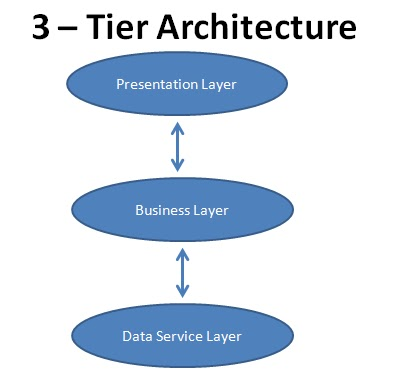
\includegraphics[width=\textwidth,
    height=0.5\textheight]{graphics/threetier.jpg}
  \caption{Ogólny schemat architektury projektowanego systemu}
\end{figure}

Każda z 3 części odpowiada za inną część związaną z procesowaniem i obsługą
zamówień:
\begin{description}
	\item[Presentation Layer] \hfill \\
		Moduł udostępniany na komputerze użytkownika, odpowiada za prezentowanie
		oferty sklepu, zbieranie akcji wykonywanych przez użytkownika i przekazywanie
		komunikacji do następnych warstw. Interfejs aplikacji
	\item[Business Layer] \hfill \\
		Moduł znajdujący się na serwerze aplikacyjnym, odpowiada za logikę całego
		systemu, koordynuje działania odpowiadające za zarządzanie zamówieniami.
		Przekazuje dane pomiędzy warstwami wyższą i niższą
	\item[Data Source] \hfill \\
		Odpowiada za trwałe przechowywanie danych a także udostępnia interfejs do ich
		pobierania, przetwarzania i zapisywania. Realizowana zazwyczaj za pomocą
		relacyjnych baz danych.
\end{description}

Dodatkowym modułem, niezbędnym w przypadku systemów, które będą wykorzystywane
przez kilkuset użytkowników jednocześnie (a taka jest docelowa przepustowość
serwerów projektowanego systemu), jest LoadBalancer, który jest odpowiedzialny
za rozkład obciążenia na osobne serwery realizujące te same funkcjonalności i
korzystające z tej samej bazy danych.

\begin{figure}[h!]
    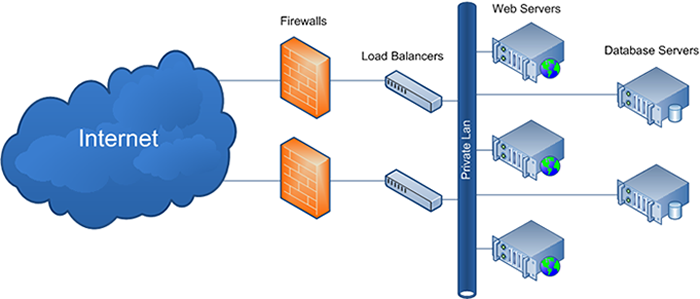
\includegraphics[width=\textwidth,
    height=0.5\textheight]{graphics/LoadBalancer.png}
  \caption{Schemat uwzględniający Load Balancer}
\end{figure}
Wybór architektury trójwarstwowej pociągnął za sobą także technologie, w których
zaimplementowane zostaną poszczególne warstwy. Z uwagi na dużą popularność, łatwość we wprowadzaniu zmian oraz wystarczająco rozbudowaną dokumentację zdecydowano się na wykorzystanie technologii JEE. Pozwala ona na stosunkowo łatwe i szybkie wdrażanie poszczególnych rozwiązań, ułatwia także zarządzanie już istniejącym projektem.

Ponieważ środowisko (zbiór technologii) Java Enterprise Edition jest bardzo
rozbudowane i posiada szereg różnych rozwiązań, konieczny stał się wybór tych
technologii, które w najlepszy sposób odwzierciedli i zapewni wsparcie dla
wymagań funkcjonalnych zdefiniowanych przez klienta. 

Zdecydowano się zatem na następujące rozwiązania technologiczne:

\begin{description}
\item[Frontend] \hfill \\
Ponieważ, jak wspomniano wcześniej, zdecydowano się na tworzenie systemu,
którego interfejs użytkownika zrealizowany jest w postaci aplikacji w
przeglądarce internetowej, wykorzystano technologie, związane z językiem Java,
które pozwalają na osadzenie w przeglądarce całej części wizualnej. W tym celu
wykorzystany zostanie wykorzystany język JavaScript wraz z technologiami HTML
oraz CSS. Pozwala to na otrzymanie wysokiej wydajności przy jednoczesnej
prostocie obsługi i implementacji. Dodatkowe funkcjonalności realizowane będą
także z wykorzystaniem biblioteki jQuery, która znacząco upraszcza proces
implementacji. Połączenie z pozostałymi warstwami obsługiwane jest z
wykorzystaniem protokołu HTTPS, co pozwala na zapewnienie bezpieczeństwa
(poprzez szyfrowanie) przekazywanych danych.
\item[Backend] \hfill \\
Jako serwer aplikacyjny zostanie wykorzystany IBM WebSphere, co pozwoli na
szybkie i łatwe implementowanie poszczególnych zależności pomiędzy modułami.
Każdy z modułów aplikacji obsługiwany jest przez zestaw Enterprise Java Beanów,
które zgromadzone są w kontenerze EJB. Komunikacja z bazą danych odbywa się z
wykorzystaniem technologii mapowania relacyjno-obiektowego zdefiniowanej w Java
Persistence API. Wybraną konkretną implementacją takiej technologii jest
framework Hibernate.
\item[Data Source] \hfill \\
Zdecydowano się na relacyjną bazę danych, które z powodzeniem są stosowane w
większości zastosowań w rozwiązaniach biznesowych i korporacyjnych od wielu lat.
Wybranym systemem bazodanowym jest Oracle w wersji 11.2. Jest to z jednej strony
najnowsza wersja systemu, pozwalająca na korzystanie z wielu obecnych tylko w
niej udogodnień a z drugiej jest to wersja stabilna, bez błędów i nieścisłości
obecnych w poprzednich edycjach wersji 11. Dane zapisywane są na zewnętrznych
macierzach dyskowych i duplikowane w celu zapewnienia bezpieczeństwa zapisu w
przypadku awarii.
\end{description}


\newpage
\begin{figure}[h!]
    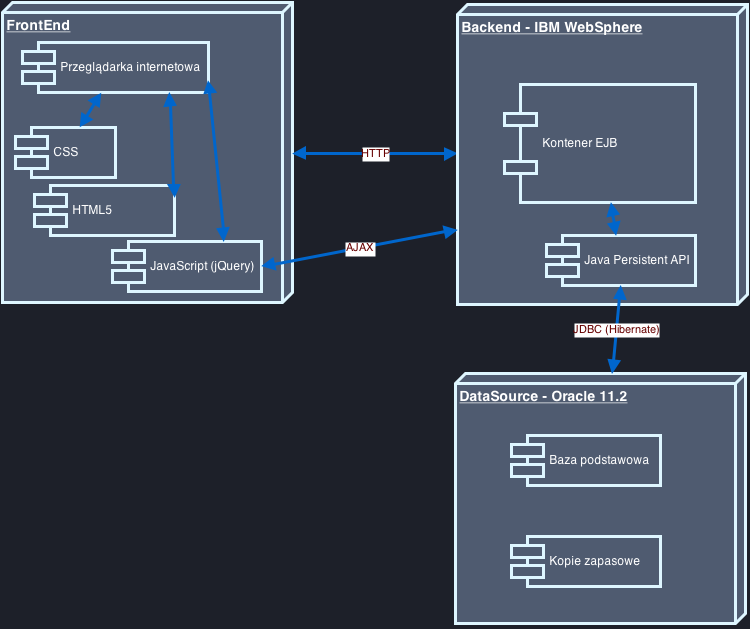
\includegraphics[width=\textwidth,
    height=0.5\textheight]{graphics/component.png}
  \caption{Architektura trójwarstwowa tworzonego systemu wraz z technologiami}
\end{figure}

Poszczegóły moduły komponentu EJB zaprezentowane są poniżej:
\begin{description}
  \item[Administracja] \hfill \\
  	Zarządzanie konfiguracją systemu, zapisem danych, umożliwienie przeglądania
  	logów
  \item[Logowanie] \hfill \\
  	Uwierzytelnianie użytkowników (klientów i pracowników) i ograniczanie lub
  	nadawanie uprawnień do poszczególnych elementów systemu
  \item[Klienci] \hfill \\
  	Obsługa informacji o klientach
  \item[Pracownicy] \hfill \\
    Obsługa informacji na temat pracowników
  \item[Części rowerowe] \hfill \\
  	Dane o częściach rowerowych, ich cenie, rozmiarze, dostępności
  \item[Zestawy rowerowe]
    Konfiguracja danych z modułu Części Rowerowe w zestawy, które mogą być
    sprzedawane całościowo
  \item[Zamówienia]
    Zarządzanie zamówieniami złożonymi przez klientów
  \item[Komunikacja klient-sklep]
    Obsługa powiadomień na temat zamówień, wymiany zapytań czy decyzji
    dotyczących zamówień
  \item[Komunikacja międzymodułowa]
    Obsługa pomiędzy pozostałymi modułami komponentu, zapis logów itp.
\end{description}


\begin{figure}[h!]
    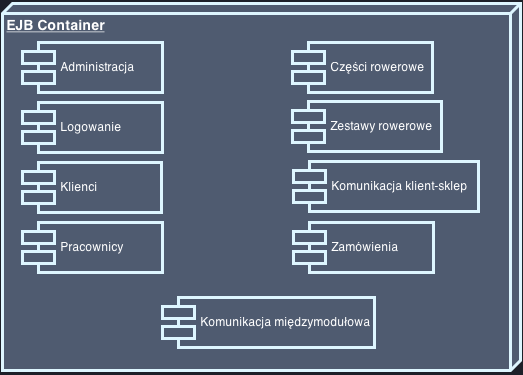
\includegraphics[width=\textwidth,
    height=0.5\textheight]{graphics/EJB.png}
  \caption{Widok szczegółowy kontenera EJB z podziałem na moduły}
\end{figure}

\subsection{Sprzęt}

Stworzenie wystarczająco jak na potrzeby niniejszego projektu rozbudowanej
infrastruktury niesie ze sobą konieczność wyboru sprzętu, na którym poszczególne
elementy składowe będą uruchomione. Ponieważ część kliencka (interfejs)
uruchamiana jest na komputerach użytkowników (klientów i pracowników) należy
podjąć decyzję co do wyboru sprzętu, na którym znajdowałby się serwer
aplikacyjny oraz serwery bazodanowe.

Jako serwer aplikacyjny zdecydowano się wykorzystać \emph{Dell PowerEdge R710}.
Charakteryzuje się on wysoką wydajnością przy jednoczesnym stosunkowo małym
poborze prądu i wysokiej jakości wykonania.

\begin{figure}[h!]
    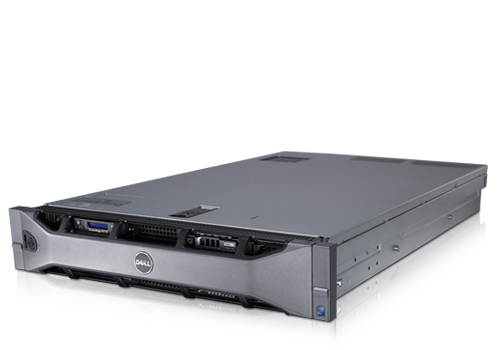
\includegraphics[width=\textwidth,
    height=0.2\textheight]{graphics/SerwerAplikacyjny.jpg}
  \caption{Wykorzystany moduł aplikacyjny}
\end{figure}

Specyfikacja techniczna serwera aplikacyjnego:

\begin{enumerate}
  \item Chipset - Intel 5520
  \item Pamięć - Do 192 GB2 (18 gniazd DIMM): 1 GB/2 GB/4 GB/8 GB/16 GB DDR3 800
  MHz, 1066 MHz lub 1333 MHz
  \item Maksymalna pojemność wewnętrznej pamięci masowej - 18 TB
  \item Gniazda - 2 PCIe x8 + 2 PCIe x4 G2 lub 1 x16 + 2 x4 G2
  \item Zasilanie - Dwa zasilacze awaryjne typu hot-plug 570 W o wysokiej sprawności ALBO dwa zasilacze awaryjne typu hot-plug 870 W o wysokiej mocy
  
\end{enumerate}


Specyfikacja bazodanowa (Oracle 11.2) wymaga także wydajnego i szybkiego
serwera, dzięki któremu dane będą zarówno pobierane jak i wstawiane w sposób
optymalny. Dlatego też zdecydowano się na serwer \emph{Dell PowerEdge R720}:

\begin{figure}[h!]
    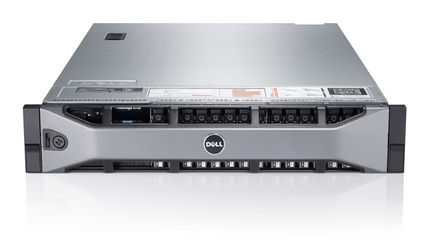
\includegraphics[width=\textwidth,
    height=0.2\textheight]{graphics/SerwerBazodanowy.jpg}
  \caption{Wykorzystany moduł bazy danych}
\end{figure}


Specyfikaczna techniczna serwera bazy danych:

\begin{enumerate}
  \item Liczba gniazd procesorów - 2
  \item Chipset - Intel C600
  \item Pamięć - Do 768 GB (24 gniazda DIMM) w modułach DDR3 2 GB/4 GB/8 GB/16
  GB/32 GB o częstotliwości do 1866 MT/
  \item Maksymalna pojemność wewnętrznej - 32 TB
  \item Gniazda - 7 gniazd PCIe:
	Jedno gniazdo x16 pełnej długości i wysokości 
	Trzy gniazda x8 pełnej długości i wysokości
	Trzy gniazda x8 o połowie długości i wysokości
  \item Zasilanie - Nadmiarowy zasilacz hot-plug o sprawności klasy Titanium i mocy 750 W
	Nadmiarowe zasilacze hot-plug o sprawności klasy Platinum i mocy 495 W, 750 W
	lub 1100 W Zasilacze z funkcją automatycznego wykrywania zakresu
\end{enumerate}


\section{Interfejs użytkownika}

W obecnych czasach niezwykle istotnym fragmentem każdego systemu sprzedaży jest
jego interfejs graficzny. Powinien być nie tylko użyteczny ale również, a może
przede wszystkich - atrakcyjny. Takie wymagania spełnia prototyp interfejsu jaki
zostanie zaprezentowany poniżej.

Cały prototyp został wykonany w technologii umożliwającej umieszczenie go w
sieci Internet pod adresem:
\url{http://rowery.hol.es/} \\
Należy jednak pamiętać, iż jest to tylko prototyp interfejsu i nie zawiera
większości funkcjonalności przyszłego systemu, a jedynie prezentuje wygląd jaki
może osiągnąć system. \\

Strona główna sklepu będzie prezentować się jak na rysunku \ref{fig:MainPage}
\begin{figure}[h!]
  \centering
    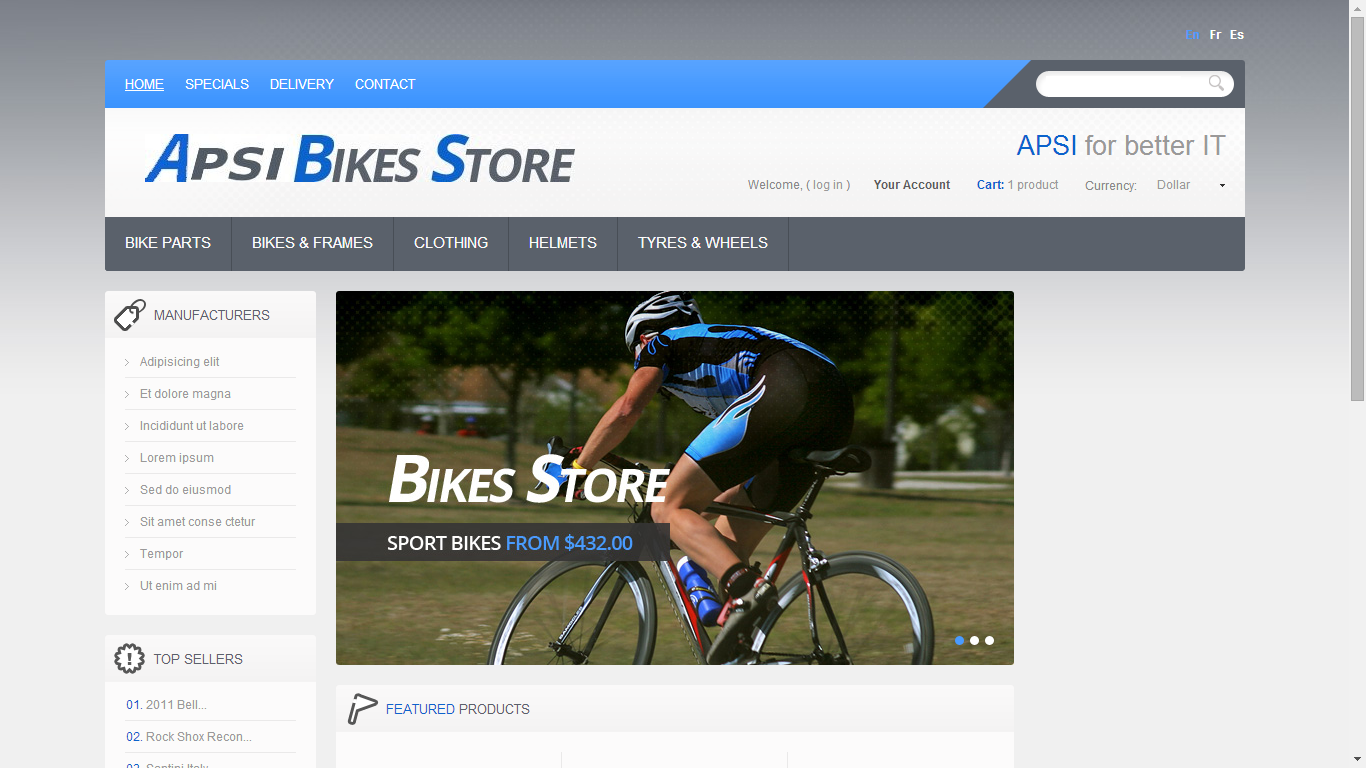
\includegraphics[width=1.0\textwidth]{graphics/ui/MainPageUp.png} 
  \caption{Strona główna sklepu}
  \label{fig:MainPage}
\end{figure}
\begin{figure}[h!]
  \centering
    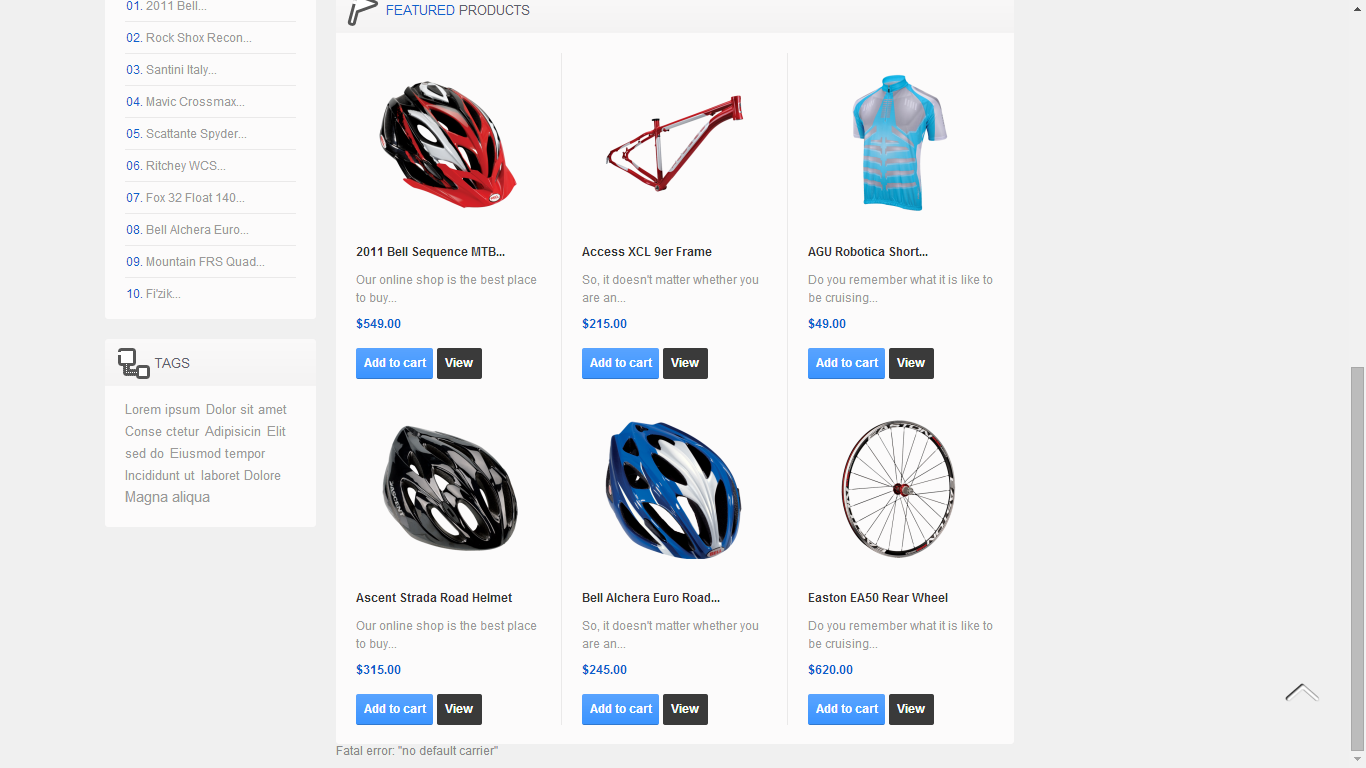
\includegraphics[width=\textwidth]{graphics/ui/MainPageBottom.png}
  \caption{Strona główna zawiera również moduł prezentujący przykładowe
  produkty}
  \label{fig:MainPageBottom}
\end{figure}

Strona główna zawiera również moduł prezentujący przykładowe produkty (Rysunek
\ref{fig:MainPageBottom}). Dzięki temu można bardzo szybko zaintersować klienta.
Sama lista produktów musi zawierać podstawowe informacje oraz zdjęcie każdego z
nich. Obrazy pozwalają na ekspresowe wybranie poszukiwanej rzeczy, natomiast
krótki opis może wystarczyć, by dodać ją do koszyka. Procedura zakupu odbywa się
przez popularny ``Koszyk''. Fragment listy produktów pokazuje Rysunek
\ref{fig:ProductList} \\

\begin{figure}[h!]
  \centering
    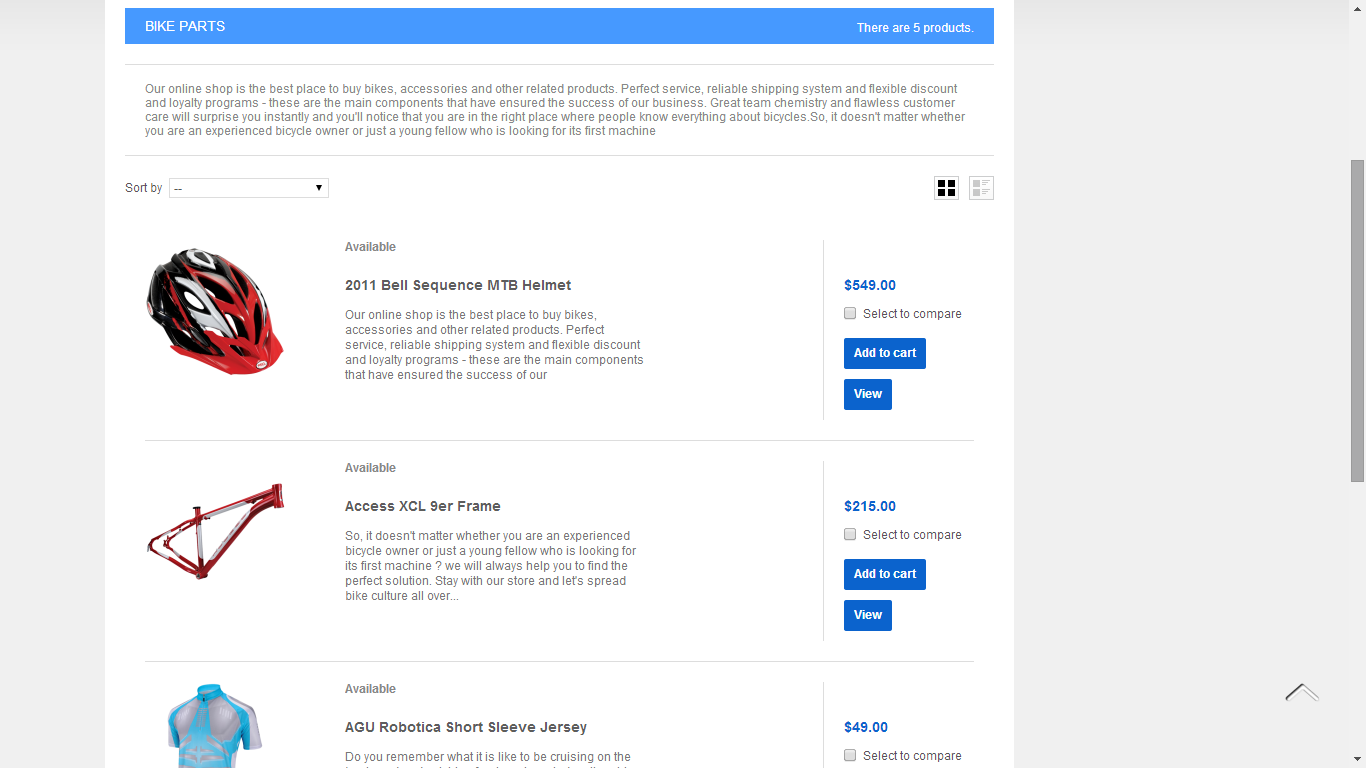
\includegraphics[width=\textwidth]{graphics/ui/Products.png}
  \caption{Fragment listy produktów}
  \label{fig:ProductList}
\end{figure}

W każdym momencie można również sprawdzić szczegóły techniczne danego produktu,
wybierając go z listy produktów, po czym użytkownik widzi nowy ekran z pełnymi
informacjami (Rysunek \ref{fig:ProductPresentation}).

\begin{figure}[h!]
  \centering
    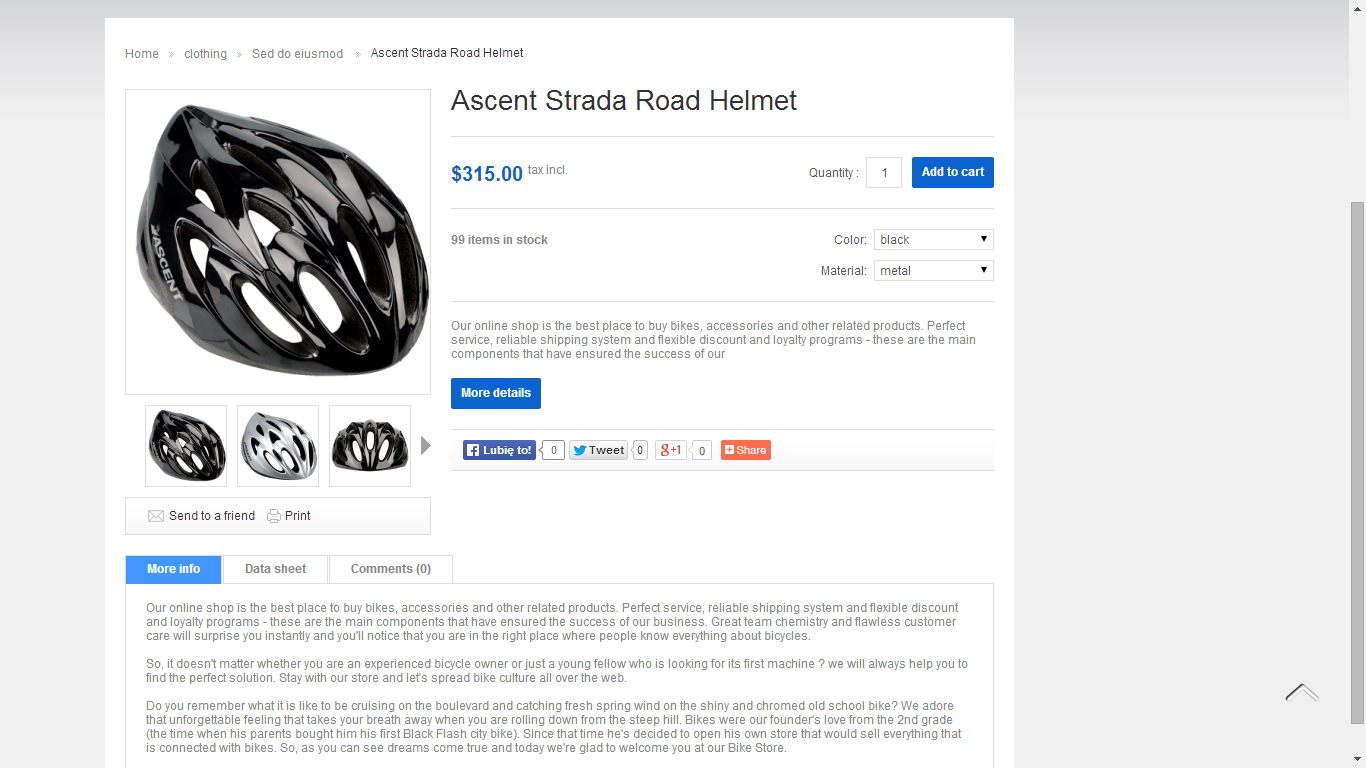
\includegraphics[width=\textwidth]{graphics/ui/ProductPresentation.png}
  \caption{Prezentacja szczegółów dotyczących produktu}
  \label{fig:ProductPresentation}
\end{figure}

\begin{figure}[h!]
  \centering
    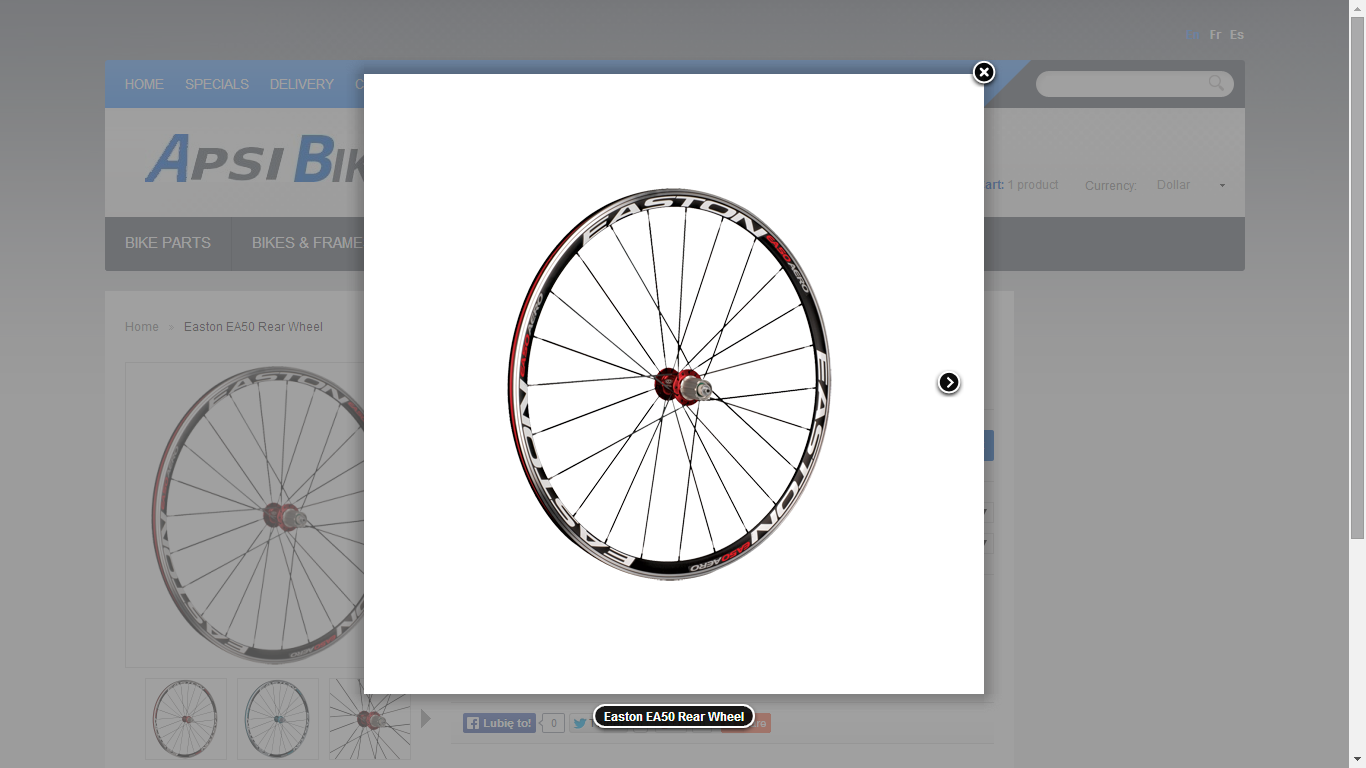
\includegraphics[width=\textwidth]{graphics/ui/ProductImage.png}
  \caption{Powiększony obraz produktu}
\end{figure}

\begin{figure}[h!]
  \centering
    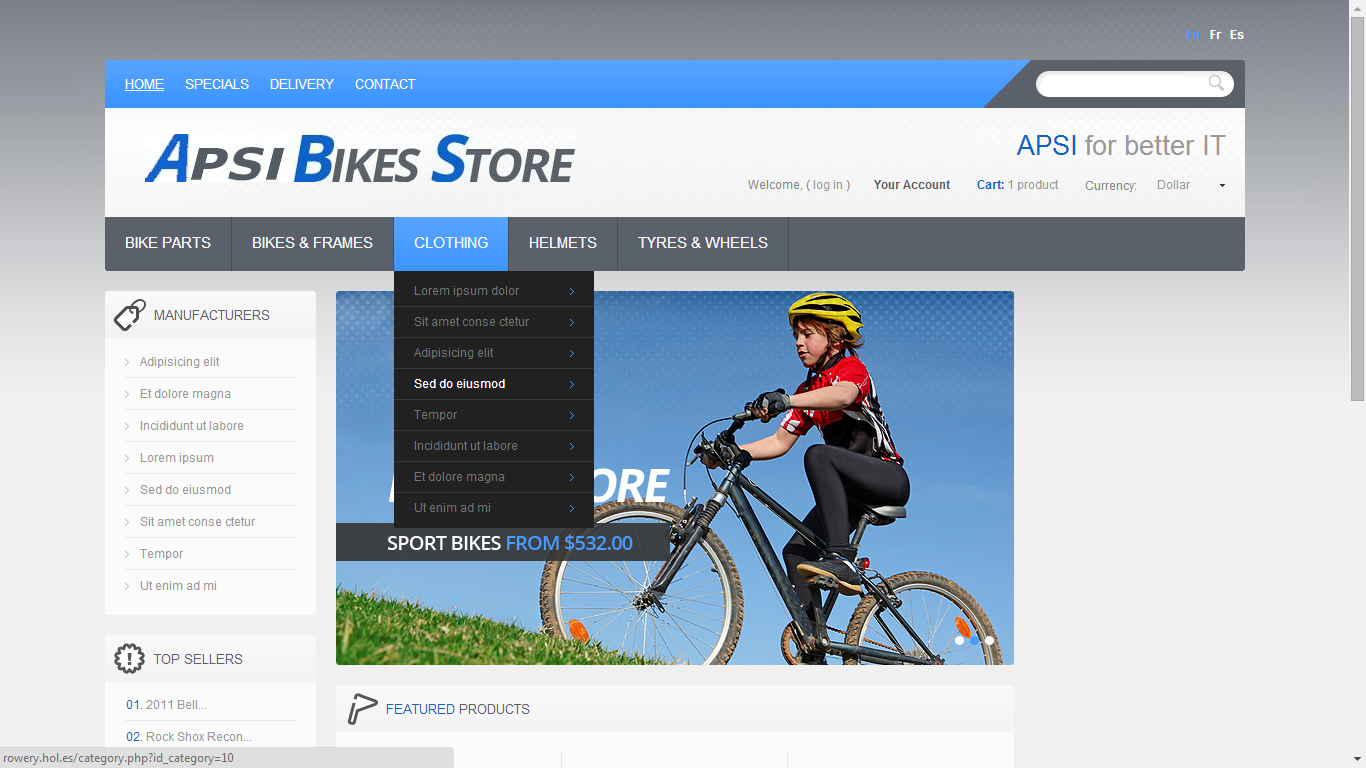
\includegraphics[width=\textwidth]{graphics/ui/MenuPresentation.png}
  \caption{Prezentacja rozwijanego menu}
\end{figure}

\begin{figure}[h!]
  \centering
    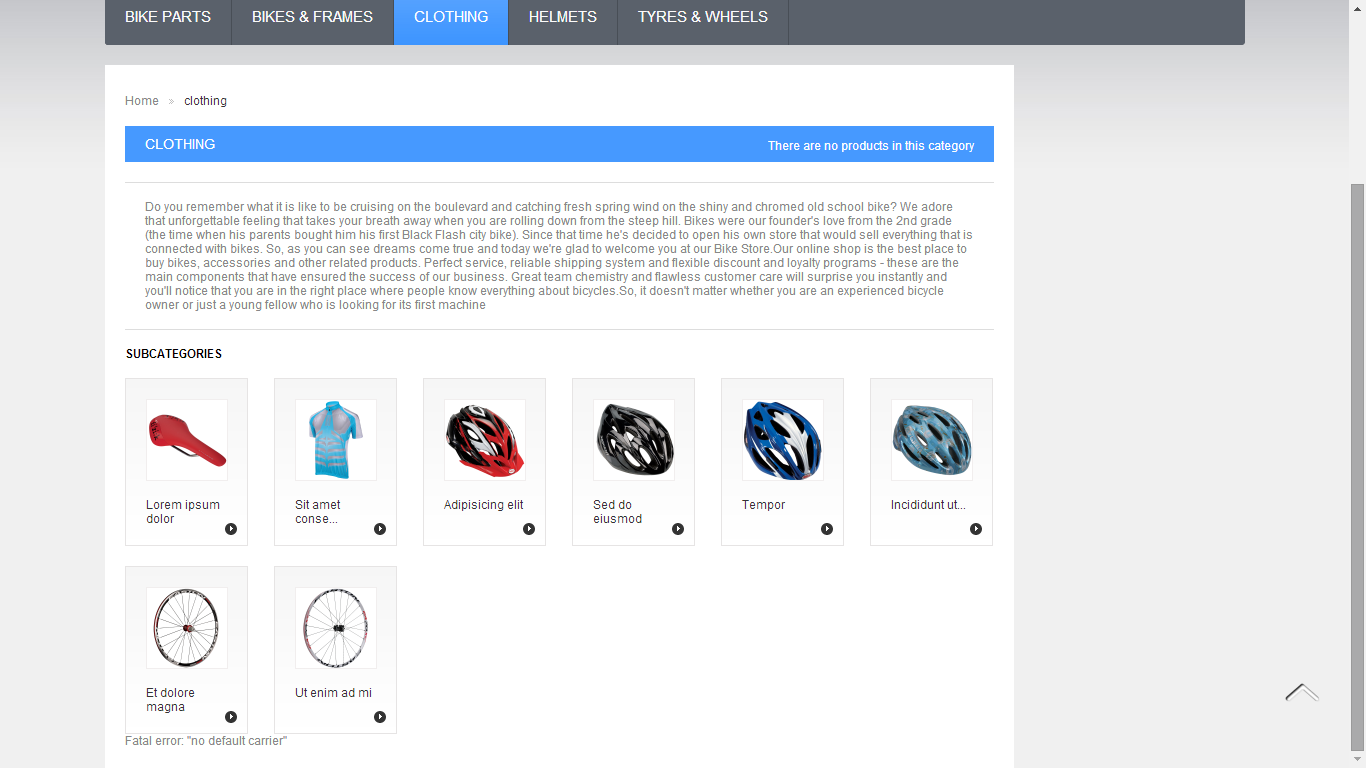
\includegraphics[width=\textwidth]{graphics/ui/Categories.png}
  \caption{Kategorie produktów}
\end{figure}

\begin{figure}[h!]
  \centering
    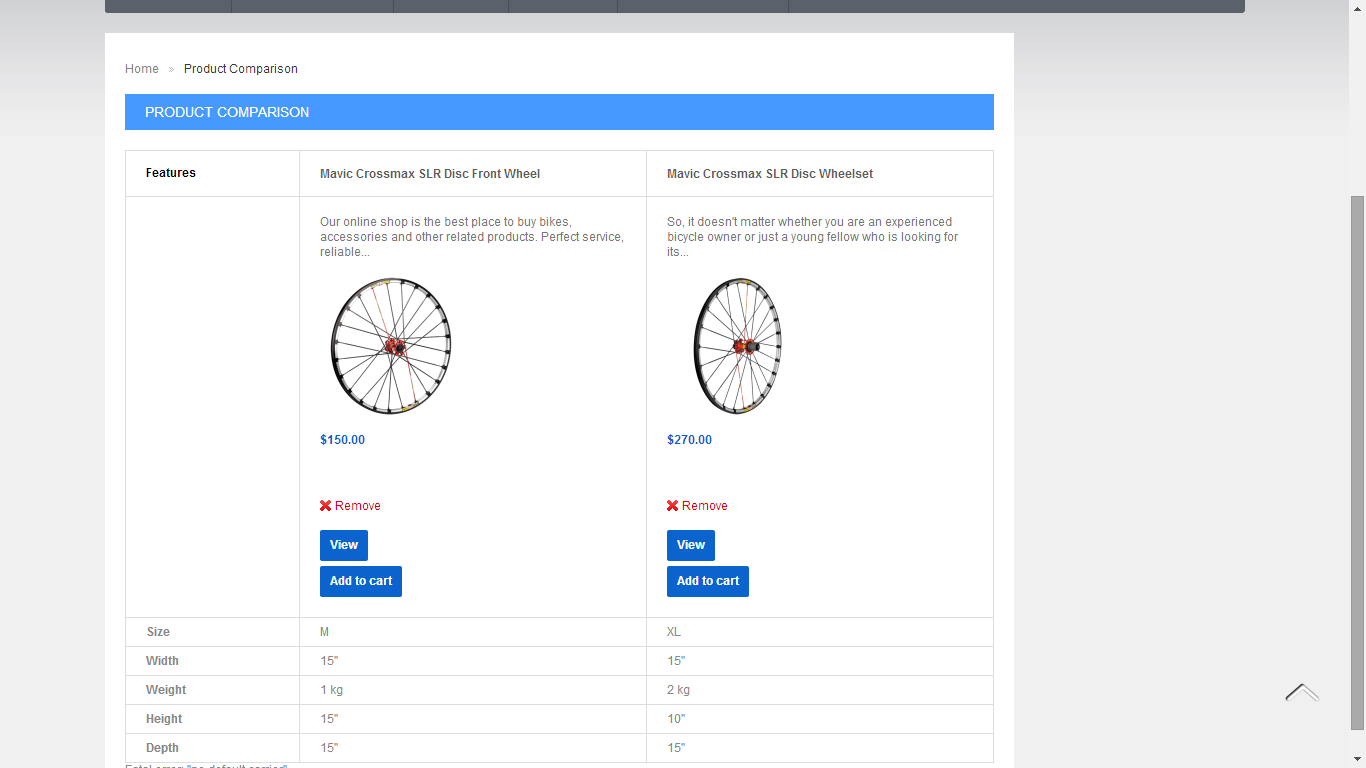
\includegraphics[width=\textwidth]{graphics/ui/ProductComparison.png}
  \caption{Porównywarka produktów}
\end{figure}
\end{document}